\documentclass[conference]{IEEEtran}
\usepackage{graphicx}
\usepackage[hidelinks]{hyperref}
\hypersetup{
  pdftitle={Instruction and Data Memory Hierarchy},
  pdfauthor={Anshuman Mehta, Rudraksh, Vridhi Chaudhary, Bineet Keshari, Shrijan Sanidhya}
}

\title{Instruction and Data Memory Hierarchy\\Design and Evaluation of a Harvard-Style Prototype}
\author{\IEEEauthorblockN{Anshuman Mehta, Rudraksh, Vridhi Chaudhary, Bineet Keshari, and Shrijan Sanidhya}
\IEEEauthorblockA{Master of Computer Applications\\Phase I Project Report}}

\begin{document}
\maketitle

\begin{abstract}
A single shared memory port serializes instruction fetches and data accesses when both are requested in the same cycle. This project implements a Verilog-2005 Harvard-style subsystem with a 16-word instruction ROM and a 16-word data RAM, each with 16-bit words. A scripted controller exercises simultaneous fetch and data operations. A 32-word single-port baseline processes the same four fetch and data request pairs using data-priority arbitration. The Harvard design completes eight memory operations in four cycles, compared with eight cycles for the baseline, yielding 2.00 and 1.00 operations per cycle, respectively. Both designs meet a 50 MHz constraint in a routed Lattice ECP5 implementation. The reported internal clock limits are 541.13 MHz for Harvard and 314.07 MHz for the shared baseline.
\end{abstract}

\begin{IEEEkeywords}
Harvard architecture, instruction memory, memory arbitration, Verilog, FPGA timing
\end{IEEEkeywords}

\section{Introduction}
Instruction fetch and operand access can contend for the same service slot in a shared-memory subsystem. This project isolates the effect of port organization with two small designs that expose the same request and response interface. Both have 32 logical word locations. The experiment varies how the locations are organized and how simultaneous requests are serviced.

A finite-state controller supplies the request sequence. Distinct ROM words make each accepted fetch observable.

\section{Literature Review}
Backus described the processor-to-store transfer path as a bottleneck in the classical von Neumann organization \cite{backus}. In the baseline used here, one address is selected per cycle. Simultaneous instruction and data requests therefore create a conflict even when the addresses refer to different regions of the array.

The Arm Cortex-M3 provides a practical example of distinct instruction and data interfaces. Its technical reference manual describes an ICode interface for instruction fetch and a DCode interface for data accesses to code space. It also recommends DCode priority when external logic arbitrates between the two \cite{arm}. Independent paths permit overlap, while a shared resource requires an explicit priority rule. The prototype isolates these mechanisms using fixed-size memories and word addresses.

Icarus Verilog separates RTL compilation and simulation through its compiler and \texttt{vvp} runtime \cite{icarus}. This supports repeatable self-checking tests and waveform inspection. Shah \emph{et al.} describe the Yosys and nextpnr flow for FPGA synthesis, placement, and routing, including the Lattice ECP5 family \cite{shah}. That flow supports a second evaluation stage in which generic gate counts and routed device timing can be interpreted independently.

\section{Proposed Solution}
\subsection{Harvard memory subsystem}
Fig.~\ref{fig:block} shows the two paths. A four-bit program counter (PC) supplies the instruction word address. It resets to zero on a rising edge, advances on an accepted fetch, and wraps from 15 to 0. The instruction ROM returns the current word combinationally. The instruction valid signal qualifies the response when fetch is enabled and reset is low.

\begin{figure}[!t]
\centering
\setlength{\unitlength}{1pt}
\begin{picture}(234,116)
\put(57,106){\makebox(0,0){\footnotesize Fetch enable}}
\put(168,106){\makebox(0,0){\footnotesize Data address and enables}}
\put(57,98){\vector(0,-1){15}}
\put(168,98){\vector(0,-1){15}}
\put(3,61){\framebox(108,22){\footnotesize 4-bit program counter}}
\put(118,61){\framebox(100,22){\footnotesize Decode and qualify}}
\put(57,61){\vector(0,-1){14}}
\put(168,61){\vector(0,-1){14}}
\put(3,25){\framebox(108,22){\footnotesize \(16\times16\) instruction ROM}}
\put(118,25){\framebox(100,22){\footnotesize \(16\times16\) data RAM}}
\put(227,84){\makebox(0,0){\scriptsize\shortstack{Write\\data}}}
\put(227,36){\line(0,1){36}}
\put(227,36){\vector(-1,0){9}}
\put(57,25){\vector(0,-1){13}}
\put(168,25){\vector(0,-1){13}}
\put(57,4){\makebox(0,0){\footnotesize Instruction word}}
\put(168,4){\makebox(0,0){\footnotesize Read data}}
\end{picture}
\caption{Harvard data flow. The controller drives both requests. Each path supplies its own valid signal, and both paths share a clock.}
\label{fig:block}
\end{figure}

\begin{figure*}[!t]
\centering
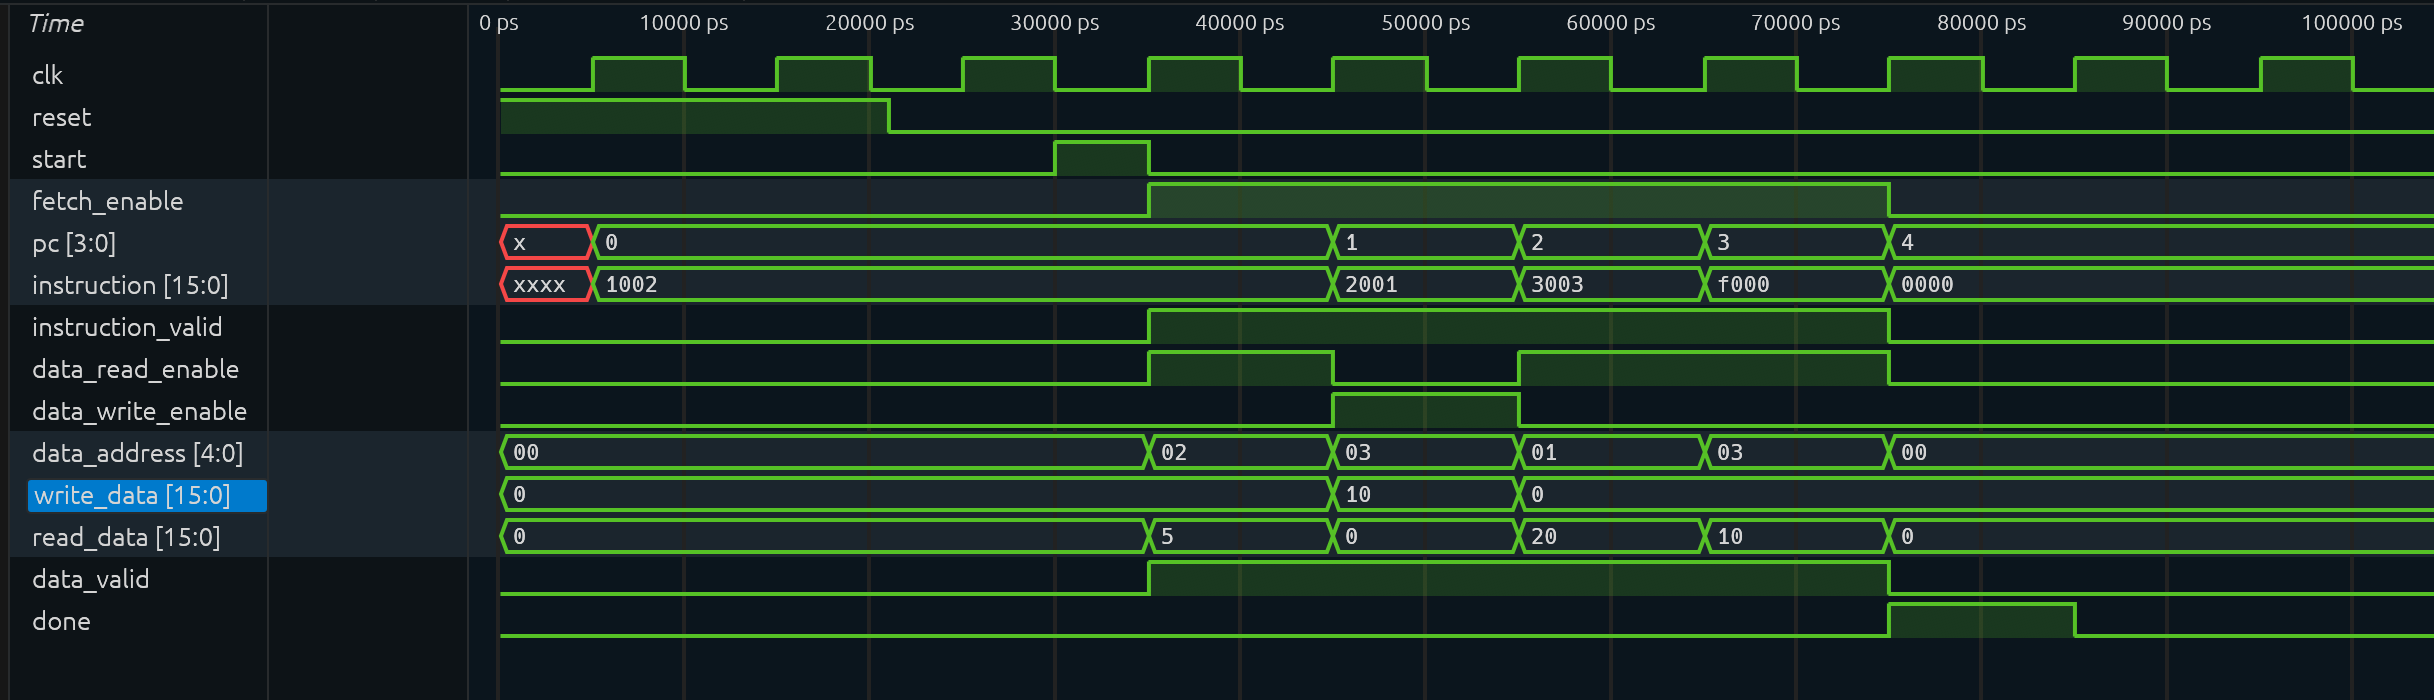
\includegraphics[width=\textwidth]{../harvard-waveform.png}
\caption{Controller-driven Harvard simulation. Fetches overlap the data read at 45 ns, write at 55 ns, and readback at 75 ns.}
\label{fig:harvard}
\end{figure*}

The data path consists of an address decoder, read/write control, and RAM. For a five-bit data address, bit 4 must be zero and the lower four bits select the word. One of read or write must be enabled for a request to be accepted. Reads return data combinationally, and writes update the selected location on the rising edge. An invalid address, conflicting enables, or reset suppresses the access. RAM contents persist across reset. The independent paths accept a fetch and a data operation on the same edge.

\subsection{Single-port baseline}
The baseline uses a 32-word array with physical addresses 0--15 assigned to instructions and 16--31 assigned to data. Both paths use the same selected address and array read. When requests coincide, a legal data access receives the port and the PC holds. The requester retains the ungranted fetch and drops the granted data request. On the next free cycle, the fetch receives the port and advances the PC. Rejected data requests leave the slot available to fetch.

\subsection{Controller and transaction sequence}
The controller moves from idle through four request states, pulses \texttt{done} for one cycle, and returns to idle. Each active state presents one fetch and one data request as shown in Table~\ref{tab:work}. The write of 10 to data word 3 is followed by a readback of 10. The other two reads check independently initialized words. Reset suppresses both transaction enables and returns the controller to idle on a rising edge.

\begin{table}[!t]
\caption{Four-pair request workload}
\label{tab:work}
\centering
\footnotesize
\setlength{\tabcolsep}{4pt}
\begin{tabular}{cclc}
\hline
PC & ROM word (hex) & Data request & Read value\\
\hline
0 & \texttt{1002} & Read word 2 & 5\\
1 & \texttt{2001} & Write 10 to word 3 & ---\\
2 & \texttt{3003} & Read word 1 & 20\\
3 & \texttt{F000} & Read word 3 & 10\\
\hline
\end{tabular}
\end{table}

\section{Verification and Results}
\subsection{Functional simulation}
All five self-checking tests passed in Icarus Verilog 13.0. The instruction and data unit tests cover PC reset, hold and wraparound, memory initialization, write timing, address range, and conflicting controls. The controller-driven test verifies four successive fetches, overlap with the data operations, readback, and the completion pulse. A direct Harvard test checks same-address isolation between ROM and RAM, a fetch during a rejected write, and RAM retention through reset. The comparison test drives each design independently and keeps each request active until its grant.

In Fig.~\ref{fig:harvard}, both valid signals are high before the 45 ns edge, where the first fetch overlaps the read of word 2. The second fetch overlaps the write of 10 to word 3 at 55 ns. The fourth fetch overlaps the readback at 75 ns, when the PC reaches 4 and \texttt{done} asserts. The waveform time axis uses picoseconds.

\subsection{Memory-access throughput}
Cycle counts start on the first request edge and end at the final grant, excluding reset and setup. In Fig.~\ref{fig:comparison}, both Harvard requests are accepted at 25 ns. The shared design grants data at 25 ns and accepts the held fetch at 35 ns. Its PC remains zero until that fetch completes. The pattern repeats for each request pair. Table~\ref{tab:performance} gives the results. The 2.00-fold throughput ratio applies to a workload that presents a fetch and a data operation together on every pair. With strict data priority, a continuous stream of legal data requests can delay a shared-port fetch until an idle slot occurs.

\begin{figure*}[!t]
\centering
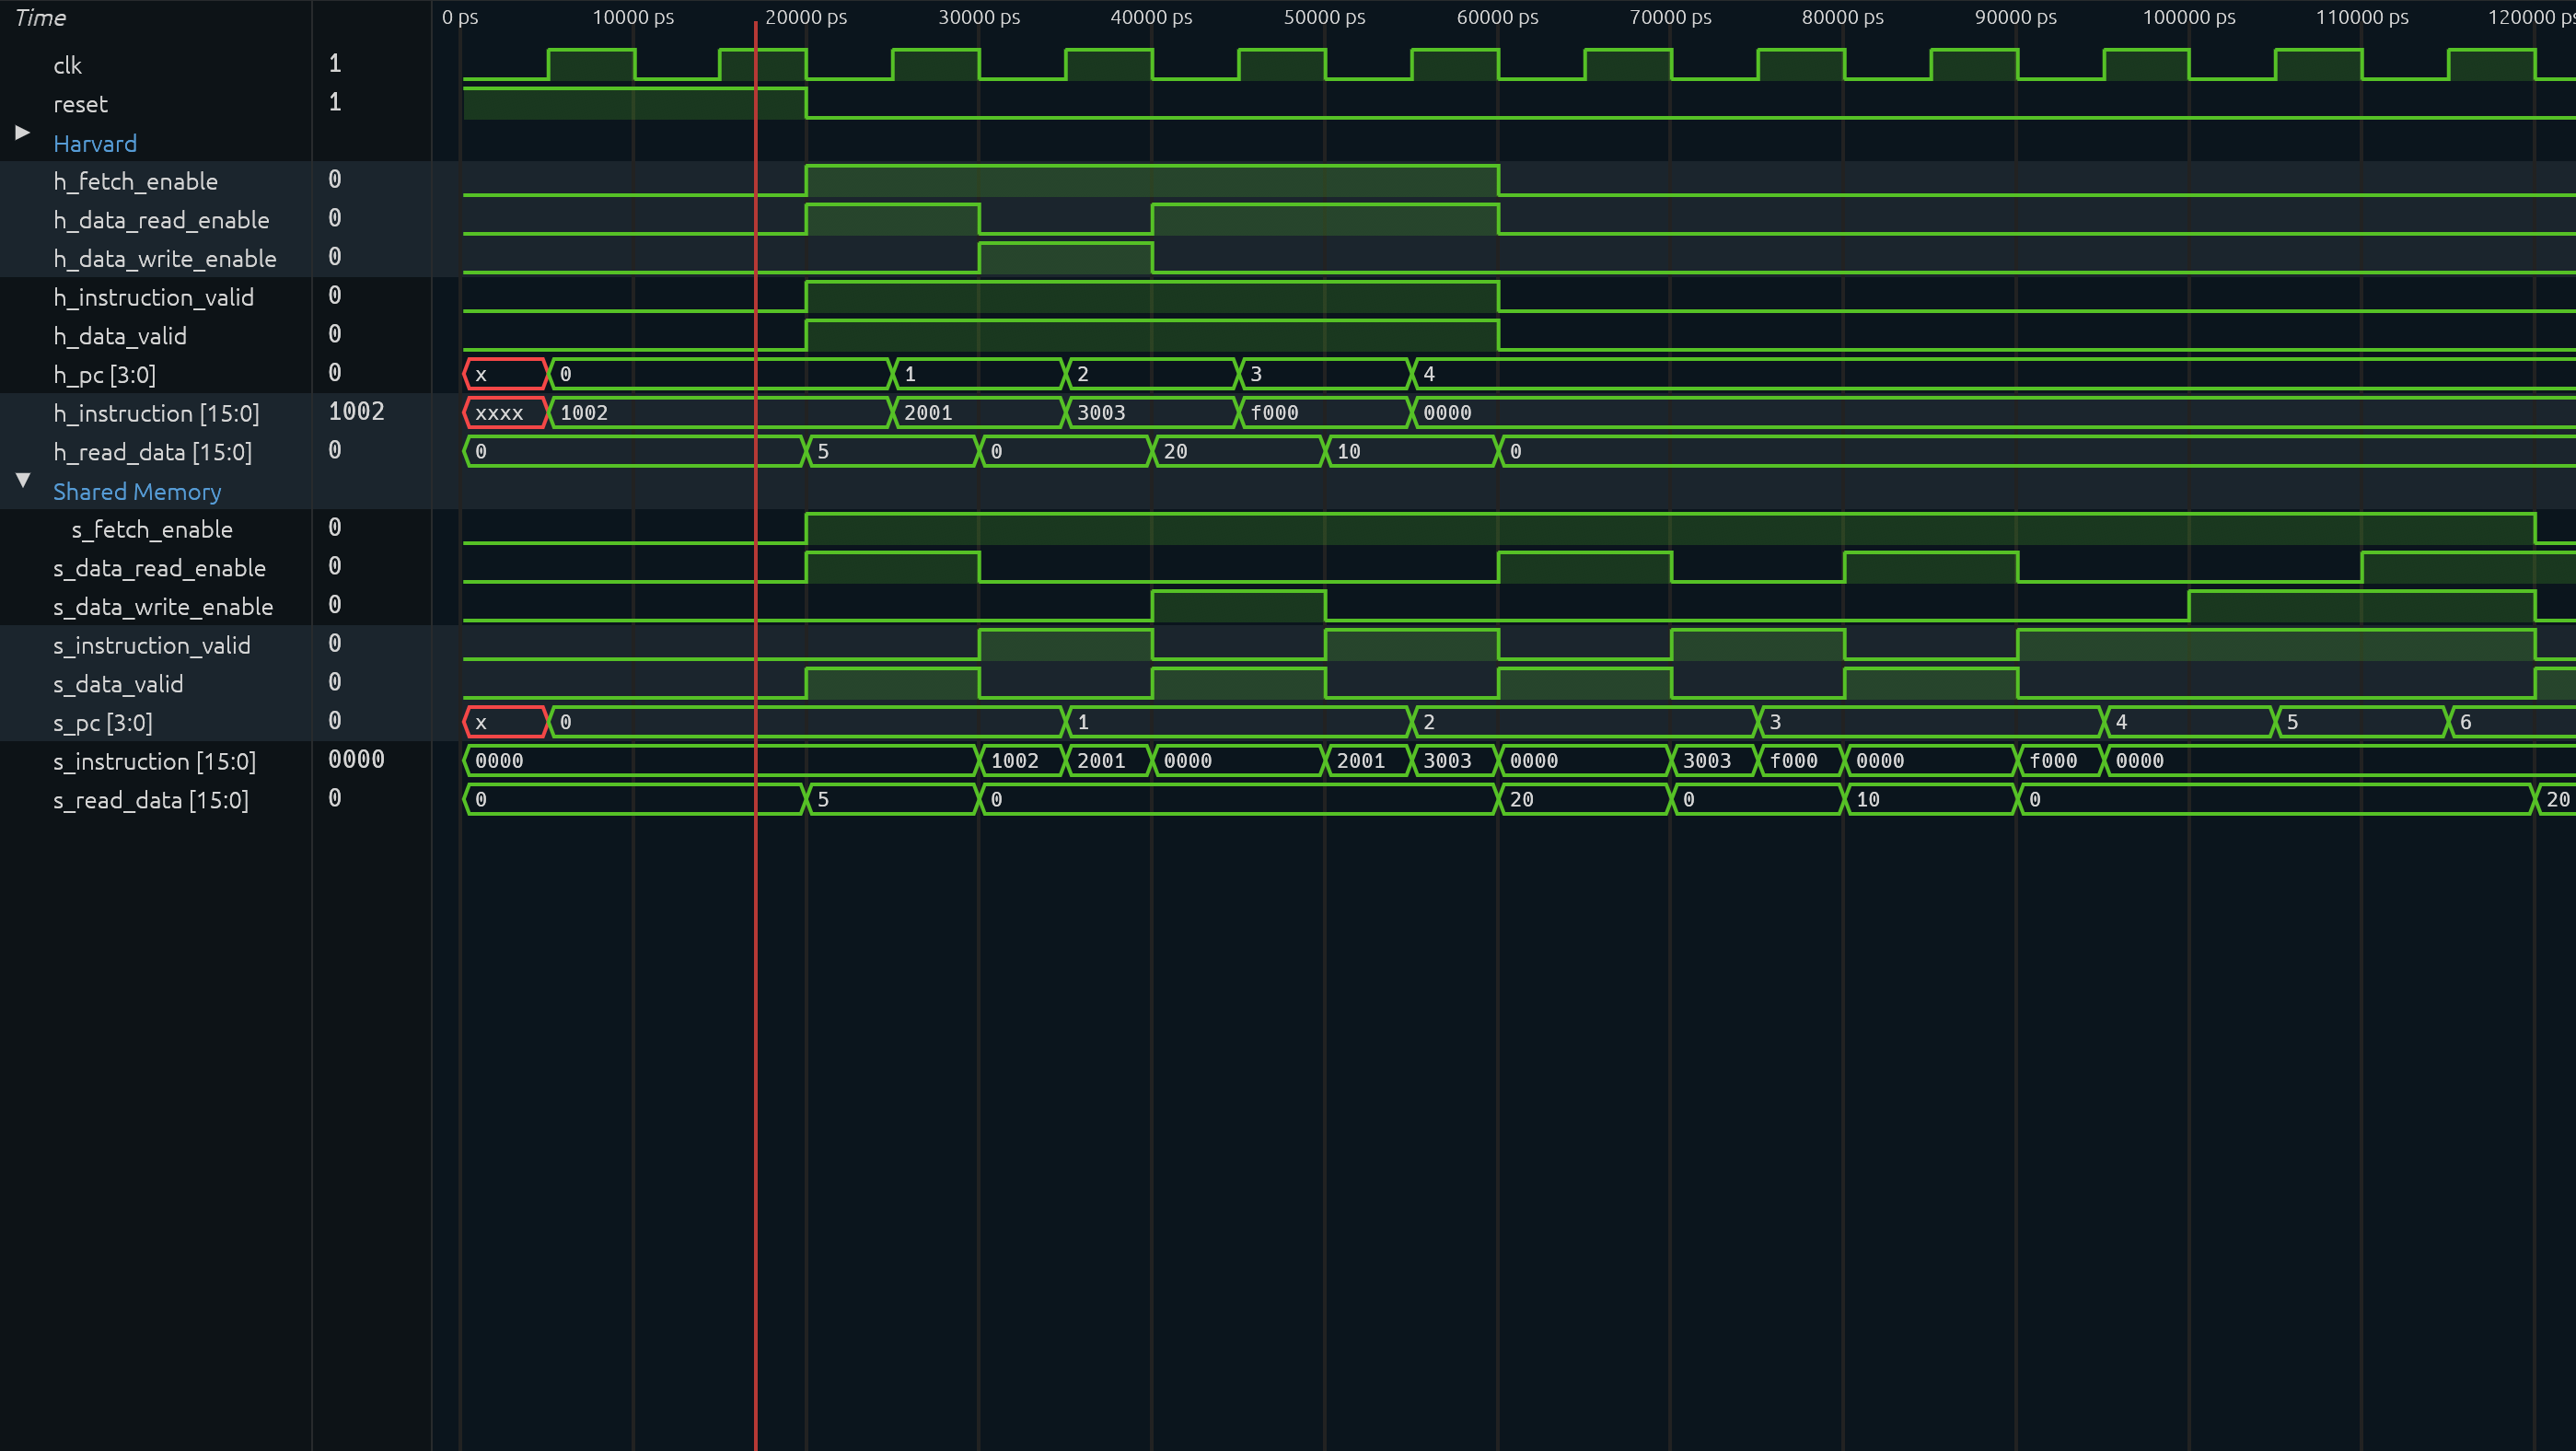
\includegraphics[width=\textwidth,trim=0 337bp 0 0,clip]{../comparison-waveform-surfer.png}
\caption{Comparison test in Surfer (1,000 ps = 1 ns). At 25 ns Harvard grants both requests while shared memory grants data. At 35 ns shared memory grants the held fetch. Readback occurs at 55 ns for Harvard and 85 ns for shared memory. Cycles after 95 ns test rejected requests.}
\label{fig:comparison}
\end{figure*}

\begin{table}[!t]
\caption{Measured memory-access performance}
\label{tab:performance}
\centering
\footnotesize
\setlength{\tabcolsep}{4pt}
\begin{tabular}{lcc}
\hline
Metric & Harvard & Shared memory\\
\hline
Accepted fetches & 4 & 4\\
Accepted data operations & 4 & 4\\
Elapsed memory-access cycles & 4 & 8\\
Operations per cycle & 2.00 & 1.00\\
Fetch stalls from contention & 0 & 4\\
\hline
\end{tabular}
\end{table}

\subsection{Synthesis and FPGA timing}
Generic Yosys synthesis reported 573 cells for Harvard and 1,217 for the shared baseline, including submodules. In that mapping the arrays use flip-flops and multiplexers. The FPGA mapping uses distributed RAM in the ECP5 programmable function units \cite{lattice}.

Both tops were synthesized with Yosys 0.70 and placed and routed with nextpnr-ecp5 0.11.1 for the LFE5U-25F, CABGA381 package, speed grade 6. The clock target was 50 MHz with placement seed 1. Table~\ref{tab:timing} reports the final post-route metrics. The longest same-clock Harvard path passes through the PC logic. The shared design has a longer path from the PC to the distributed RAM write-address logic.

\begin{table}[!t]
\caption{ECP5 post-route timing and utilization}
\label{tab:timing}
\centering
\footnotesize
\setlength{\tabcolsep}{4pt}
\begin{tabular}{lcc}
\hline
Metric & Harvard & Shared memory\\
\hline
50 MHz clock constraint & Pass & Pass\\
Internal clock \(F_{\max}\) (MHz) & 541.13 & 314.07\\
Longest same-clock path (ns) & 1.85 & 3.18\\
Longest input-to-output path (ns) & 8.20 & 10.35\\
Combinational sites & 69 & 104\\
Flip-flops & 4 & 4\\
Distributed RAM write sites & 4 & 8\\
Block RAMs & 0 & 0\\
\hline
\end{tabular}
\end{table}

The \(F_{\max}\) values apply to internal clock paths. The tool assigned I/O pins automatically and used no board-specific external timing constraints. The 10 ns simulation clock is a stimulus setting. The project repository includes the RTL, testbenches, waveforms, and raw timing reports~\cite{repo}.

\section{Individual Contributions}
\textbf{Anshuman Mehta} defined the interfaces and implemented the PC, ROM, and Harvard top. He verified integration, ran ECP5 timing, and prepared the report.

\textbf{Rudraksh} implemented the decoder, read/write control, RAM, and data-path wrapper. His unit tests covered valid access, aliasing, conflicts, and reset retention.

\begin{samepage}
\textbf{Vridhi Chaudhary} implemented the controller and Harvard integration test. She documented the waveform showing concurrent fetch and data access, including write readback.\par
\end{samepage}

\textbf{Bineet Keshari} implemented the single-port baseline and arbitration, wrote the matched-workload benchmark, captured the comparison waveform, and documented the throughput and generic Yosys synthesis results.

\textbf{Shrijan Sanidhya} implemented the direct Harvard testbench. His tests cover same-address ROM and RAM isolation, fetch progress during a rejected write, and RAM retention when reset suppresses active requests.

\begin{thebibliography}{00}
\bibitem{backus}
J. Backus, \textquotedblleft Can programming be liberated from the von Neumann style? A functional style and its algebra of programs,\textquotedblright\ \emph{Commun. ACM}, vol.~21, no.~8, pp.~613--641, Aug. 1978, doi: \href{https://doi.org/10.1145/359576.359579}{10.1145/359576.359579}.

\bibitem{arm}
Arm Limited, \emph{Cortex-M3 Technical Reference Manual}, rev.~r2p1, ARM DDI 0337I, 2010. [Online]. Available: \href{https://www.keil.com/dd/docs/datashts/arm/cortex_m3/r2p1/ddi0337i_cortexm3_r2p1_trm.pdf}{Arm Cortex-M3 Technical Reference Manual}.

\bibitem{icarus}
Icarus Verilog Project, \textquotedblleft Getting started with Icarus Verilog,\textquotedblright\ \emph{Icarus Verilog Documentation}. [Online]. Available: \href{https://steveicarus.github.io/iverilog/usage/getting_started.html}{Icarus Verilog Getting Started Guide}.

\bibitem{shah}
D. Shah, E. Hung, C. Wolf, S. Bazanski, D. Gisselquist, and M. Milanovi\'{c}, \textquotedblleft Yosys+nextpnr: An open source framework from Verilog to bitstream for commercial FPGAs,\textquotedblright\ in \emph{Proc. IEEE Int. Symp. Field-Programmable Custom Computing Machines (FCCM)}, 2019, pp.~1--4, doi: \href{https://doi.org/10.1109/FCCM.2019.00010}{10.1109/FCCM.2019.00010}.

\bibitem{lattice}
Lattice Semiconductor, \emph{ECP5 and ECP5-5G Family Data Sheet}, FPGA-DS-02012, rev.~3.0, 2022. [Online]. Available: \href{https://www.latticesemi.com/-/media/LatticeSemi/Documents/DataSheets/ECP5/FPGA-DS-02012-3-0-ECP5-ECP5G-Family-Data-Sheet.ashx?document_id=50461}{Lattice ECP5 Family Data Sheet}.

\bibitem{repo}
A. Mehta, Rudraksh, V. Chaudhary, B. Keshari, and S. Sanidhya, \textquotedblleft Instruction and data memory hierarchy,\textquotedblright\ project repository, commit \texttt{d481e00}, 2026. [Online]. Available: \url{https://github.com/Anshuman-utd/MCA_Project/tree/d481e00}.
\end{thebibliography}

\end{document}
